Your introduction here.
Include some references~\cite{derivative_of_polynomials_via_double_limit,
    alekseyev2018mathoverflow,
    oeis_coefficients_u_m_l_k_defined_by_polynomial_identity_3}.
Lorem Ipsum is simply dummy text of the printing and typesetting industry.
Lorem Ipsum has been the industry's standard dummy text ever since the 1500s, when an unknown printer took a galley
of type and scrambled it to make a type specimen book.
It has survived not only five centuries, but also the leap into electronic typesetting, remaining essentially unchanged.
It was popularised in the 1960s with the release of Letraset sheets containing Lorem Ipsum passages, and more
recently with desktop publishing software like Aldus PageMaker including versions of Lorem Ipsum.

Figure example
\begin{figure}[H]
    \centering
    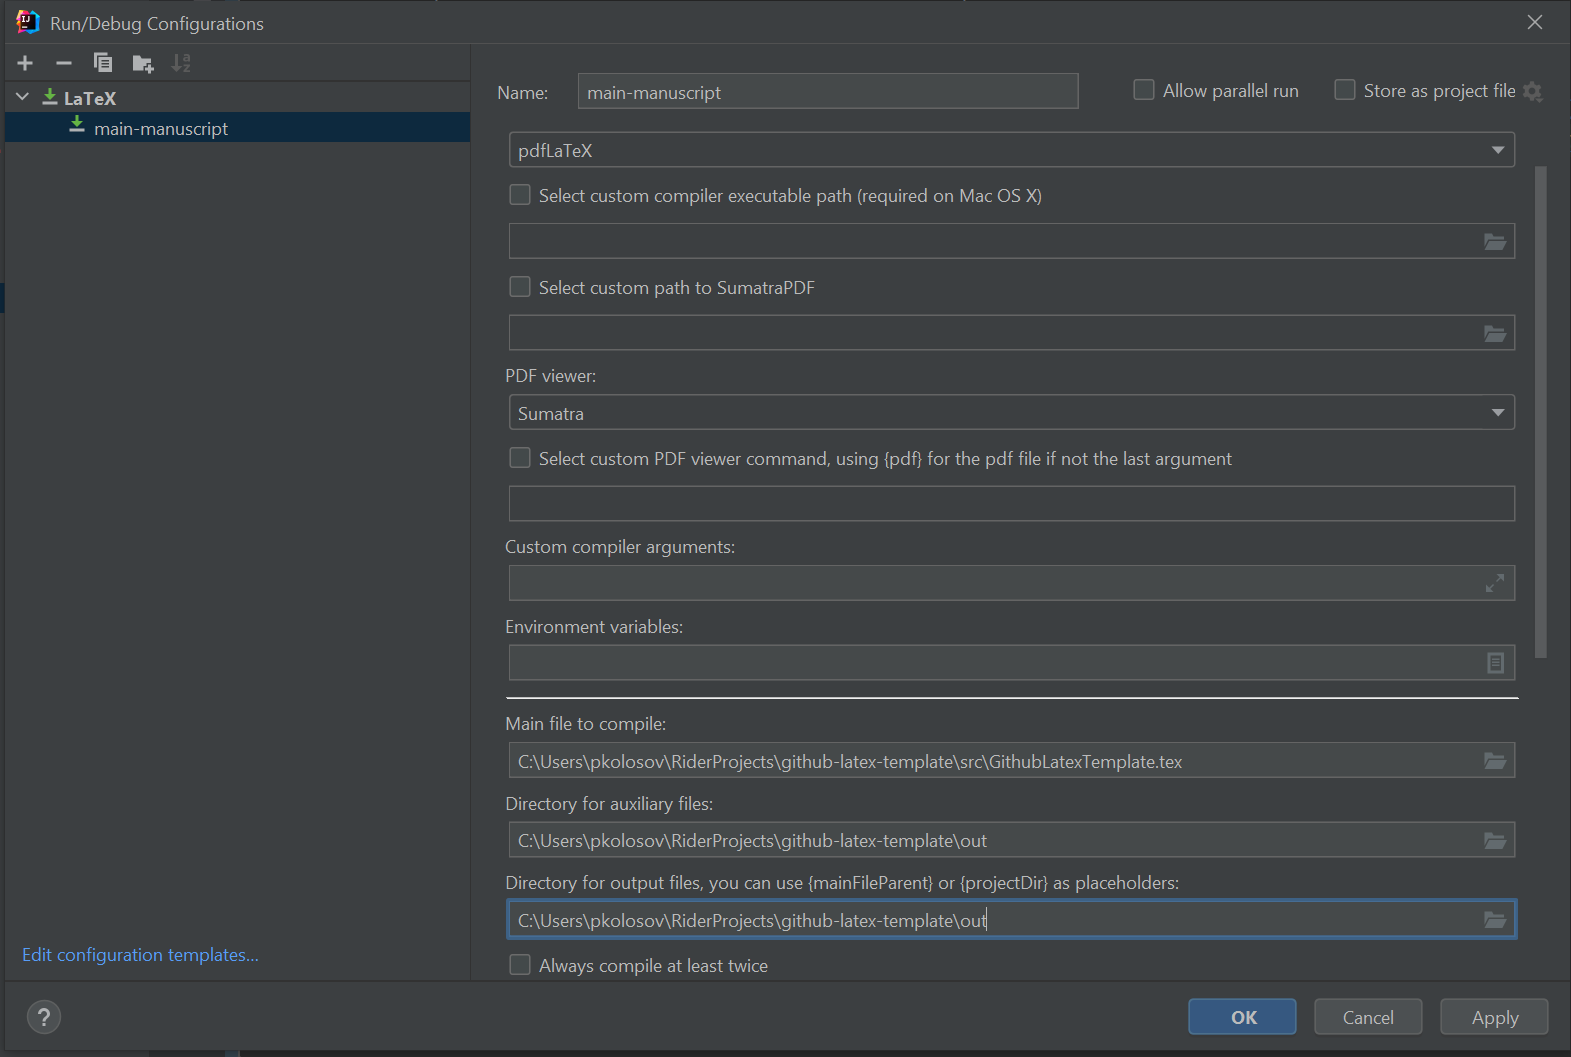
\includegraphics[width=1\textwidth]{sections/images/latex_configuration}
    ~\caption{Figure example.}\label{fig:figure}
\end{figure}

\begin{table}[H]
    \begin{center}
        \setlength\extrarowheight{-6pt}
        \begin{tabular}{c|cccccccc}
            $m/r$ & 0 & 1       & 2      & 3      & 4   & 5    & 6     & 7 \\ [3px]
            \hline
            0     & 1 &         &        &        &     &      &       &       \\
            1     & 1 & 6       &        &        &     &      &       &       \\
            2     & 1 & 0       & 30     &        &     &      &       &       \\
            3     & 1 & -14     & 0      & 140    &     &      &       &       \\
            4     & 1 & -120    & 0      & 0      & 630 &      &       &       \\
            5     & 1 & -1386   & 660    & 0      & 0   & 2772 &       &       \\
            6     & 1 & -21840  & 18018  & 0      & 0   & 0    & 12012 &       \\
            7     & 1 & -450054 & 491400 & -60060 & 0   & 0    & 0     & 51480
        \end{tabular}
    \end{center}
    \caption{Coefficients $\coeffA{m}{r}$. See OEIS sequences
    ~\cite{oeis_numerators_of_the_coefficient_a_m_r,oeis_denominators_of_the_coefficient_a_m_r}.}
    \label{tab:table_of_coefficients_a}
\end{table}


\begin{equation*}
    \llceil \nobarfrac{a}{b} \rrfloor_{m}
\end{equation*}
\begin{equation*}
    \llceilCoefficient{a}{b}{m}
\end{equation*}

And for any natural $m$ we have polynomial identity
\begin{equation}
    x^m = \sum_{k=1}^{m} T(m, k) \centralFactorial{x}{k}
    \label{eq:knuth-power-identity}
\end{equation}
where $\centralFactorial{x}{k}$ denotes central factorial defined by
\begin{equation*}
    \centralFactorial{x}{n} = x \fallingFactorial{x+\frac{n}{2}-1}{n-1}
\end{equation*}
where $\fallingFactorial{n}{k} = n (n-1) (n-2) \cdots (n-k+1)$ denotes falling factorial in Knuth's notation.
In particular,
\begin{equation}
    \centralFactorial{x}{n}
    = x \left( x+\frac{n}{2}-1 \right) \left( x+\frac{n}{2}-1 \right) \cdots \left (x+\frac{n}{2}-n-1 \right)
    = x \prod_{k=1}^{n-1} \left( x+\frac{n}{2}-k \right)\label{eq:equation}
\end{equation}
